\input{setup/preamble.tex}% package inclusion and set up of the document

%%%%%%%%%%%%%%%%%%%%%%%%%%%%%%%%%%%%%%%%%%%%%%%%%%%%%
%             UNITS, EQUATIONS AND TEXT             %
%%%%%%%%%%%%%%%%%%%%%%%%%%%%%%%%%%%%%%%%%%%%%%%%%%%%%
%Units:
\newcommand{\unit}[1]{&& \left[\si{#1}\right]} %\newcommand{\unit}[1]{[\si{#1}]}             <<| Use these if you want equations to be
\newcommand{\unitWh}[1]{[\si{#1}]}             %\newcommand{\eq}[2]{&&\si{#1} &= \si{#2}&&}  <<| centered.. .. will appear scrambled
\newcommand{\numUnit}[1]{\ \si{#1}&}           %                                               | from one equation to the next though..
%Equation:                                     %                                               | and does not work with long equations.. :/
\newcommand{\eq}[2]{\si{#1} &= \si{#2}}
\newcommand{\arw}{&& &\Updownarrow&&}
%Text:
\newcommand{\tx}[1]{\text{#1}}
%Vectors
\renewcommand{\vec}[1]{\boldsymbol{\mathbf{#1}}}
%Vertical line in equations ie. |_x=y (whereTwo stacks two equalities at the line)
\newcommand{\where}[1]{ \left.\rule{0cm}{.5cm}\right\vert\rule{0cm}{.4cm}_{\substack{\rule{0cm}{.15cm}\\ \si{#1} }} }
\newcommand{\whereTwo}[2]{ \left.\rule{0cm}{.67cm}\right\vert\rule{0cm}{.5cm}_{\substack{\si{#1} \rule{0cm}{.19cm}\\\vspace{-.1cm}\\ \si{#2}}} }

%%%%%%%%%%%%%%%%%%%%%%%%%%%%%%%%%%%%%%%%%%%%%%%%%%%%%
%                  REFERENCES                       %
%%%%%%%%%%%%%%%%%%%%%%%%%%%%%%%%%%%%%%%%%%%%%%%%%%%%%

%Chapter
\newcommand{\Chapref}[1]{\emph{Chapter \ref{#1}}}
\newcommand{\chapref}[1]{\emph{chapter \ref{#1}}}
%Section
\newcommand{\Secref}[1]{\emph{Section \ref{#1}}}
\newcommand{\secref}[1]{\emph{section \ref{#1}}}
%subSection
\newcommand{\Subsecref}[1]{\emph{Subsection \ref{#1}}}
\newcommand{\subsecref}[1]{\emph{subsection \ref{#1}}}
%Appendix
\newcommand{\Appref}[1]{\emph{Appendix \ref{#1}}}
\newcommand{\appref}[1]{\emph{appendix \ref{#1}}}
%Listings
\newcommand{\Coderef}[1]{\emph{Listings: \ref{#1}}}
\newcommand{\coderef}[1]{\emph{listings: \ref{#1}}}
%Figure:
\newcommand{\Figref}[1]{\emph{Figure \ref{#1}}}
\newcommand{\figref}[1]{\emph{figure \ref{#1}}}
%Table:
\newcommand{\Tableref}[1]{\emph{Table \ref{#1}}}
\newcommand{\tableref}[1]{\emph{table \ref{#1}}}

%Expressions:
\newcommand{\Expr}[1]{\emph{Expression (\ref{#1})}}
\newcommand{\expr}[1]{\emph{expression (\ref{#1})}}

%Equations:
%1 equation:
\newcommand{\Eqref}[1]{\emph{Equation (\ref{#1})}}
\renewcommand{\eqref}[1]{\emph{equation (\ref{#1})}}
%2 equations:
\newcommand{\EqrefTwo}[2]{\emph{Equation (\ref{#1})} and \emph{(\ref{#2})}}
\newcommand{\eqrefTwo}[2]{\emph{equation (\ref{#1})} and \emph{(\ref{#2})}}
%3 equations:
\newcommand{\EqrefThree}[3]{\emph{Equation (\ref{#1})}, \emph{(\ref{#2})} and \emph{(\ref{#3})}}
\newcommand{\eqrefThree}[3]{\emph{equation (\ref{#1})}, \emph{(\ref{#2})} and \emph{(\ref{#3})}}
%4 equations:
\newcommand{\EqrefFour}[4]{\emph{Equation (\ref{#1})}, \emph{(\ref{#2})}, \emph{(\ref{#3})} and \emph{(\ref{#4})}}
\newcommand{\eqrefFour}[4]{\emph{equation (\ref{#1})}, \emph{(\ref{#2})}, \emph{(\ref{#3})} and \emph{(\ref{#4})}}
%5 equations:
\newcommand{\EqrefFive}[5]{\emph{Equation (\ref{#1})}, \emph{(\ref{#2})}, \emph{(\ref{#3})}, \emph{(\ref{#4})} and \emph{(\ref{#5})}}
\newcommand{\eqrefFive}[5]{\emph{equation (\ref{#1})}, \emph{(\ref{#2})}, \emph{(\ref{#3})}, \emph{(\ref{#4})} and \emph{(\ref{#5})}}
%6 equations:
\newcommand{\EqrefSix}[6]{\emph{Equation (\ref{#1})}, \emph{(\ref{#2})}, \emph{(\ref{#3})}, \emph{(\ref{#4})}, \emph{(\ref{#5})} and \emph{(\ref{#6})}}
\newcommand{\eqrefSix}[6]{\emph{equation (\ref{#1})}, \emph{(\ref{#2})}, \emph{(\ref{#3})}, \emph{(\ref{#4})}, \emph{(\ref{#5})} and \emph{(\ref{#6})}}
%7 equations:
\newcommand{\EqrefSeven}[7]{\emph{Equation (\ref{#1})}, \emph{(\ref{#2})}, \emph{(\ref{#3})}, \emph{(\ref{#4})}, \emph{(\ref{#5})}, \emph{(\ref{#6})} and \emph{(\ref{#7})}}
\newcommand{\eqrefSeven}[7]{\emph{equation (\ref{#1})}, \emph{(\ref{#2})}, \emph{(\ref{#3})}, \emph{(\ref{#4})}, \emph{(\ref{#5})}, \emph{(\ref{#6})} and \emph{(\ref{#7})}}% my new macros

\begin{document}
%%% Prereport %%%
\setlength\cftaftertoctitleskip{2pt}
\setlength\cftafterloftitleskip{6pt}
\setlength\cftafterlottitleskip{6pt}
\selectlanguage{english}
\title{Cubli}

%%% Frontmatter Settings %%%
\pagestyle{empty} %disable headers and footers
\pagenumbering{roman} %use roman page numbering in the frontmatter I II...
\fancyfoot[RE,LO]{15gr510} %page number on all pages
\fancyfoot[LE,RO]{\thepage}
\fancyhead[LE,LO,RE,RO]{}

%%% Introductory Formalities %%%
%\includepdf[pages={1}]{formalities/frontpage.pdf}
%\pdfbookmark[0]{Front Page}{label:forside}%
\begin{titlepage}
  \addtolength{\hoffset}{0.5\evensidemargin-0.5\oddsidemargin} %set equal margins on the frontpage - remove this line if you want default margins
  \noindent%
  \begin{tabular}{@{}p{\textwidth}@{}}
    \toprule[2pt]
    \midrule
    \vspace{0.2cm}
    \begin{center}
    \Huge{\textbf{
      Autonomous Lawn Mower % insert your title here
    }}
    \end{center}
    \begin{center}
      \Large{
      Utilizing a Local Positioning System
      }
    \end{center}
    \vspace{0.2cm}\\
    \midrule
    \toprule[2pt]
  \end{tabular}
   \vspace{0.55 cm}
  \begin{figure}[!ht]
\centering
\includegraphics[width=0.8\textwidth]{figures/frontPageImage.pdf}
\label{fig:forside}
\end{figure}
  \vspace{-0.35 cm}
  \begin{center}
    {\large
      5. Semester Project Report %Insert document type (e.g., Project Report)
    }\\
    \vspace{0.2cm}
    {\Large
      Group 15gr510%Insert your group name or real names here
    }
  \end{center}
  \begin{center}
  Aalborg University\\
  Electronic Engineering \& IT\\
  Fredrik Bajers Vej 7\\
  DK-9220 Aalborg
  \end{center}
\end{titlepage}

\clearpage
\pagestyle{fancy}
{\small
\strut\vfill % push the content to the bottom of the page
\noindent Copyright \copyright{} Aalborg University 2015\par
\vspace{0.2cm}

\noindent This report is compiled in \LaTeX, originally developed by Leslie Lamport, based on Donald Knuth's \TeX. The main text is written in \emph{Latin Modern} pt 12, designed by Bogusław Jackowski and Janusz M. Nowacki. 
%The document is compiled via the website \url{www.overleaf.com}, an online collaborative based \LaTeX-editor with instant preview, which enables multiple persons to edit the document simultaneously.
Flowcharts and diagrams are made using Microsoft Visio. 
\clearpage
%\begin{document} 
%\thispagestyle{empty}
%\begin{titlepage}
\begin{nopagebreak}
{\samepage 

\begin{tabular}{r}
\parbox{\textwidth}{  \raisebox{-15mm}{\includegraphics[height=3cm]{figures/aaulogo-en.png}}
\hfill \hspace{2cm} \parbox{8cm}{\begin{tabular}{l} %4.90
{\small \textbf{\textcolor{aaublue}{\colorbox{white}{6\textsuperscript{th} Semester, Bachelor Project}}}}\\
{\small \textbf{\textcolor{aaublue}{School of Information and}}}\\
{\small \textbf{\textcolor{aaublue}{Communication Technologies}}}\\ 
{\small \textbf{\textcolor{aaublue}{Electronics and IT}}}\\
{\small \textcolor{aaublue}{Fredrik Bajers Vej 7C}} \\
{\small \textcolor{aaublue}{9220 Aalborg}} \\
{\small \textcolor{aaublue}{\emph{http://www.sict.aau.dk/electronics-and-it}}}
\end{tabular}}}
\end{tabular}

\begin{tabular}{cc}
\parbox{7cm}{

\textbf{Title:}

Cubli:\\
Dynamic Control of a Reaction Wheel Inverted Pendulum\\ %\fxnote{Input project title}\\

\textbf{Theme:}

\small{
BSc Project (Control Engineering)\\
}


\parbox{8cm}{


\textbf{Project Period:}\\
P6, Spring 2016\\
01/02/2016 - 25/05/2016\\
   
\textbf{Project Group:}\\
630\\ %\fxnote{Input group number}
  
\textbf{Participants:}\\
Bjørn Kitz\\
Julien Br\'ehin\\
Mikael Sander\\
Niels Skov Vestergaard\\
Noelia Villarmarzo Arruñada\\

\textbf{Supervisors:}\\
John-Josef Leth\\ %\fxnote{Input supervisor}
Palle Andersen
}\\

\textbf{Prints:} 8\\
\textbf{Pages:} 125\\
\textbf{Appendices:} 15 (37 pages)\\
\textbf{Attached:} 1 DVD\\
\textbf{Concluded:} 25/05/2016\\

\vfill } &
\parbox{7cm}{
  \vspace{.15cm}
  \hfill
  \begin{tabular}{l}
  {\textbf{Synopsis}}\bigskip \\
  \fbox{
    \parbox{6.5cm}{\bigskip
     {\vfill{\small The inverted pendulum is used in many applications and it is a classic research area in control theory which is still active.

The aim of this project was to model and analyze the behavior of a reaction wheel inverted pendulum, in the form of a one-frame Cubli; and to design a controller capable of balancing it in equilibrium position. 

A controller was designed using classical control methods such as root locus and Nyquist criterion. However, the system had a marginally stable behavior. Not having control of the velocity of the reaction wheel was a problem, so the final controller was done through state space design.

Moreover, a solution for measuring its angular position using only internally mounted sensors was designed to be able to make it portable to a full Cubli. 

Finally, the performance of the system was tested on the prototype to ensure that it fulfills the needed requirements.
     \bigskip}}
     }}
   \end{tabular}}
\end{tabular}} %\vspace{1cm}

\textit{\phantom{A}Publication of this report's contents (including citation) without permission\\ \phantom{A}from the authors is prohibited}\\

\end{nopagebreak}
%\end{titlepage}
%\end{document}
%%% Preface %%%
%\cleardoublepage
\textbf{\huge{Preface}}
\\
\\
The purpose of this project is to design and implement a control system that can maintain a reaction wheel inverted pendulum in upright position using only internally mounted sensors.

This report has been written by a group of students on the sixth semester of "Electronics and IT" at Aalborg University.
The reader should have a basic knowledge on Electronic Engineering, specially in Modeling and Control Theory, and Convex Optimization, although specific topics will be described in more detail. Code for the implementation is written in C++ and the reader is assumed to be able to comprehend this programming language. 

Thanks:\\
- Simon Jensen, assistant engineer, Department of Electronic Systems, Aalborg University \\
- Simon Vestergaard Johansen, Business Ph.d., worked with the cubli previously, discussed project with us,\\
- Benjamin Krebs, former AAU student, wrote the base code for the cubli, has provided help.\\
- Thanks to our supervisors John-Josef Leth and Palle Andersen

\textbf{Reading Instructions}
\\
\\
The report is structured in three parts:
\begin{itemize}
\item[-] Part I contains an analysis of the system, which includes a description of the given setup, the derivation of the dynamic model and the acquisition of the parameters of the system.
\item[-] Part II deals with the design and implementation of the controller and the complementary filter used to measure the angular position of hte frame.
\item[-] Part III includes the acceptance tests made to the system and the conclusions that can be derived from the project.
\end{itemize}

The attached CD contains a digital copy of this report, all the data and Matlab files needed to plot the figures in the report, datasheets, the code needed to run the controller, the code needed for the implementation of the optimization, the Senstools manual and a video of the working system.  

\textbf{Text by:}\\
\vspace{-12 pt}
\begin{table}[H]
	\centering
		\begin{tabular}{c c c}
			\underline{\phantom{JAERJAERJAERJAERGO}} & \phantom{cookies} & \underline{\phantom{JAERJAERJAERJAERGO}} \\
			Bjørn Kitz			& \phantom{cookies} & Julien Br\'ehin		\\
			&&\\
			\underline{\phantom{JAERJAERJAERJAERGO}} & \phantom{cookies} & \underline{\phantom{JAERJAERJAERJAERGO}} \\
			Mikael Sander			& \phantom{cookies} & Niels Skov Vestergaard		\\
			&&\\
	    \multicolumn{3}{c}{\underline{\phantom{JAERJAERJAERJAERGO}}}\\
	    \multicolumn{3}{c}{Noelia Villarmarzo Arruñada}\\				
		\end{tabular}
\end{table}
\pagebreak

\pdfbookmark[0]{Table of Contents}{label: tableOfCentents}
\tableofcontents
\cleardoublepage


%%% Mainmatter Settings %%%
\pagenumbering{arabic} %use arabic page numbering in the mainmatter
\fancyfoot[RO,LE]{\thepage \text{ of} \pageref{LastPage}}
\fancyfoot[RE,LO]{15gr510}
\fancyhead[RE,LO]{}
\fancyhead[RE,LO]{\color{aaublue}\small\nouppercase\leftmark} %even page - chapter title
\pagestyle{fancy}

%%% Part 1 %%%
\part{Preanalysis}

%---------- Chapter 1 ---------------------------------------- Introduction
%\chapter{Introduction}\label{introduction}
The effective control of an inverted pendulum is still an active area of research nowadays. \cite{JHuber}

One type of this kind of systems is a setup called Cubli. It consists of a cube controlled with reaction wheels. The Cubli can jump up and balance on one of its edges or on one of its corners, as shown in \figref{CubliCorner}.
The Cubli is designed as a simple setup to let control engineers work with an inverted pendulum. A working Cubli can also be an interesting way to show and explain the general public  what control engineering is about. \cite{MGajamohan}
%
\begin{figure}[H] 
	\centering
	\includegraphics[scale=1.3]{figures/CubliCorner-700x430}
	\caption{A Cubli balancing on one of its corners\cite{RAndrea}}
	\label{CubliCorner}
\end{figure}
%
Applications for this cube robot, that moves without any external tools, might seem limited when you only have a single cube. However, if you take a group of cubes, they could move together to traverse obstacles or solve puzzles one cube alone could not. A group of cubes can form a structure (\figref{MBlocksExample}), and by talking in between each other they can use their reaction wheels to get the structure to move in the desired direction. Since each cube can move independently, a single cube can detach for an assignment or catch up with the main structure if it gets dropped. \cite{JRomanishin}
%
\begin{figure}[H] 
	\centering
	\includegraphics[scale=0.4]{figures/m-blocks}
	\caption{A number of cube robots (called M-blocks at Massachusetts Institute of Technology (MIT)) shown making two different structures. These M-blocks stick together with the help of magnets placed in their corners \cite{LRosen}}
	\label{MBlocksExample}
\end{figure}
%
It has also been suggested using similar technology for alternative locomotion in planetary or asteroid exploration. The internal actuation is not very efficient in high gravity environments, however, in environments with microgravity such as asteroids the technology becomes very feasible. \cite{RAllen}

In microgravity a Cubli could tumble or even jump across the surface. A traditional rover with wheels would not be able to sufficiently grip or might even push the rover off the surface long enough for it to land upside down. Where such a situation would be fatal for most rovers, a cube with internal actuation would not be immobilized by landing upside down.\cite{ELandau}

This concept was the basis of a small experimental lander called MINERVA, short for Micro/Nano Experimental Robot Vehicle for Asteroids, which were to explore the near earth asteroid Itokawa (see \figref{MINERVA}). The lander was deployed from its mother spacecraft HAYABUSA in 2005, when it unfortunately missed the asteroid's small gravitational pull and drifted off into space. \cite{TYoshimitsu}
%
\begin{figure}[H] 
	\centering
	\includegraphics[scale=.8]{figures/MINERVA}
	\caption{MINERVA experimental lander, which was designed for asteroid exploration \cite{TYoshimitsu}}
	\label{MINERVA}
\end{figure}
%
A more recent example of development in this area is NASA's Hedgehog robot, which also is actuated internally with reaction wheels. It has bee through several tests aboard an aircraft for microgravity research in June 2015, where it showed its ability to jumping out of a sandpit. A picture of the Hedgehog robot can be seen in \figref{Hedgehog}. \cite{ELandau}
%
\begin{figure}[H] 
	\centering
	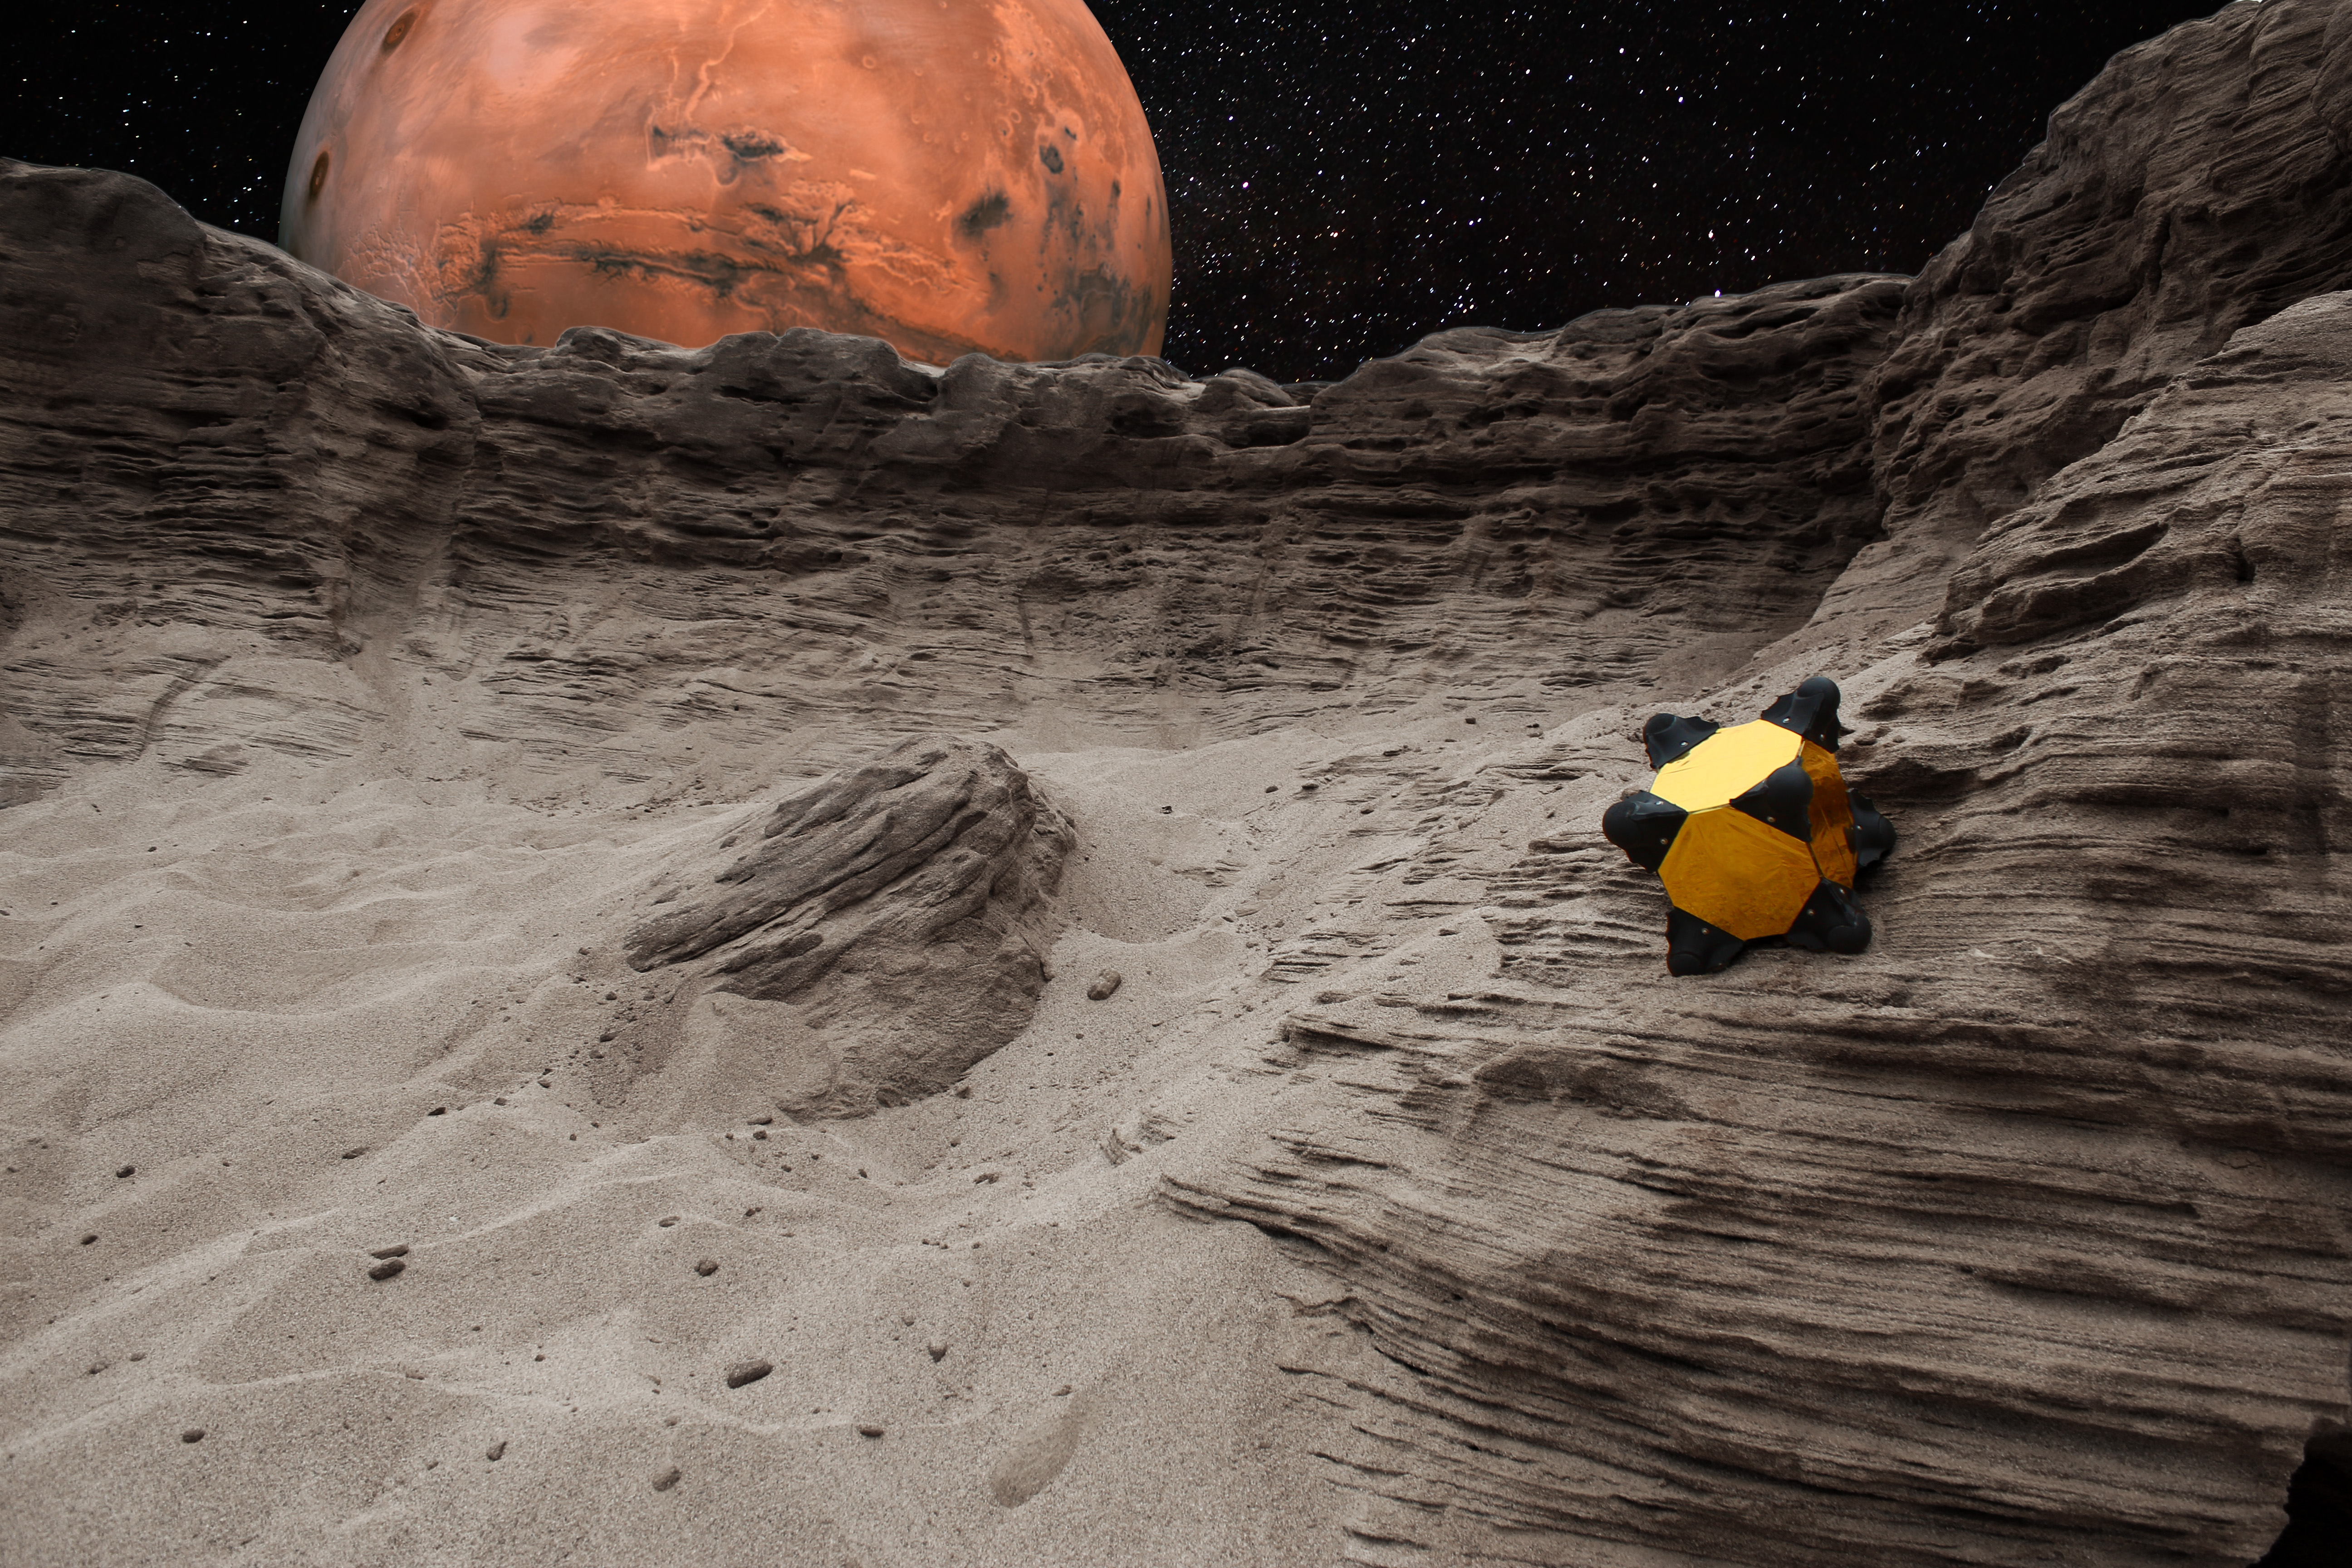
\includegraphics[scale=0.05]{figures/Hedgehog}
	\caption{NASA's Hedgehog robot for asteroid exploration \cite{ELandau}}
	\label{Hedgehog}
\end{figure}
%\section{AAU Cubli}
Here at AAU there was build a one-dimensional model of the cubli. It is fixed to an axis with one of its corners, so it can rotate around that corner, but cannot be moved translational.

The AAU cubli consists of the following parts\fxnote{insert correct part names}.

\begin{table}[H]
	\begin{tabular}{|l|p{3.8cm}|}
		\hline %-----------------------------------------------------------------------------------
		\textbf{No.} &\textbf{Part} 			\\
		\hline %-----------------------------------------------------------------------------------
		1            & Frame           			\\
		\hline %-----------------------------------------------------------------------------------
		2            & Reaction wheel      		\\
		\hline %-----------------------------------------------------------------------------------
		3            & IMU           			\\
		\hline %-----------------------------------------------------------------------------------
		4            & BeagleBone           	\\
		\hline %-----------------------------------------------------------------------------------
		5            & Potentiometer           	\\
		\hline %-----------------------------------------------------------------------------------
		6            & Motorcontrolboard    	\\
		\hline %-----------------------------------------------------------------------------------
		7            & Brushless DC-motor    	\\
		\hline %-----------------------------------------------------------------------------------
		8            & Jump brake		    	\\
		\hline %-----------------------------------------------------------------------------------
	\end{tabular}
	\caption{Table over parts in the Cubli setup \label{TableAAUCubliComponent}}
\end{table}

\subsection{Subsection 1.1.1}
The frame is made of metal? \fxnote{find composition of frame if possible} and is mainly a square with a solid edge at the outer bound of the frame, and two cross connections between opposing corners. 

The reaction wheel is a wheel made of metal? \fxnote{find composition of wheel if possible} with most of the mass in a ring at its outer edge and two crossconnections, that are going trough its center at rigth angle to each other. It is connected with the motor and the frame through and axis going throught its center of rotation.


The BeagleBone recieves the data from sensors and motor and with the control algorithm uploaded to it, tries to balance the cubli, by spinning up the reaction wheel.

The potentiometer is placed at the corner of the frame that is fixed to an axis. It is used to measure the angel of the frame.

The motor spins up the reaction wheel and also brakes it during the balancing part of the controller. When jumping up the cubli the motor will spin up the reaction wheel and the jump brake will then suddenly brake the reaction wheel.
\subsection{Subsection 1.1.2}
%\input{chapters/chapter1/cSectionAndSubsections.tex} %-------- For Overview, somtimes short headlines here works well

%---------- Chapter 2 ---------------------------------------- Design Considerations
\chapter{Design Considerations}
The setup for this project is given by the university, which means that some considerations must be taken into account when modeling the system and designing a controller to balance it.

%---------- Chapter 3 ---------------------------------------- Requirements
%\section{Design Limitations}
The working setup that exists at Aalborg University (AAU) is composed by one of the sides of the 3D cube.

Since all the hardware is already build, the goal of the project is focus on deriving the model of the system, simulate it to compare it with the real Cubli and design a controller capable of balance it in the equilibrium position.

One important characteristic is that one of its corners is attached to a base plate. This feature limits the number of movements the Cubli can do, as it can only be balance in one direction.

Another important limitation is given by the maximum current that the motor can provide which conditions the maximum starting angle that it can have with respect to equilibrium position. As can be seen in \figref{}, if the initial angle is different from 0 rad both the mass of the frame ans the mass of the wheel exert an initial torque to the system. This must be overcame by the motor in order to the Cubli not to fall.
%
\begin{figure}[H] 
	\centering
	\includegraphics[scale=0.65]{figures/limitationTorque}
	\caption{Force acting on the system that create an initial torque}
	\label{limitationTorque}
\end{figure}

The minimum torque that the motor must apply is give by \eqref{minTorque}.
%
\begin{flalign}
	\eq{T} { (m_F \cdot l_F + m_w \cdot l_w) \cdot g \cdot sin(\theta_F)} \unit{N\cdot m}
	\label{minTorque}
\end{flalign}

Since the torque is restricted by the characteristics of the motor and the control board, the maximum initial angle is derived in \eqref{maxAngle}.
%
\begin{flalign}
	\eq{\theta_F} { asin\left(\frac{T}{(m_F \cdot l_F + m_w \cdot l_w) \cdot g}\right)} \unit{N\cdot m}
	\label{maxAngle}
\end{flalign}
%
Substituding the values of the maximum torque (see section \ref{sec:Motor}) and the parameters of the Cubli (see section \ref{sec:Param}) the maximum starting angle is \si{0,2024\ rad}.

\fxnote{The maximum angle may should be explained after the modeling and the estimation of parameters}
%At Aalborg University (AAU), there exists a working setup of a one-dimensional Cubli. The overall goals of this semester are to make a model of a system, to simulate this model and then to design and implement a controller for that system. Students on this semester are encouraged to work with pre-made setups, since the focus is rather on the control engineering than the hardware solution.\fxnote{moved the section directly from introduction. Will need a top to catch the previous chapter}



%%% Part 2 %%%
\part{Design \& Implementation}
%---------- Chapter 4 ---------------------------------------- Modelling
\chapter{System Description}\label{systemDescription}
One-frame Cubli is a non-linear unstable system which is capable of laying on one of its corners as long as it is properly controlled, using the inertia created in the reaction wheel present in the setup.



This system is composed by several hardware parts, listed in the following table. \fxnote{Include picture of the real model, mark all the parts in the picture}

\begin{table}[H]
	\begin{tabular}{|l|p{6.7cm}|}
		\hline %-----------------------------------------------------------------------------------
		\textbf{No.} &\textbf{Part} 			\\
		\hline %-----------------------------------------------------------------------------------
		1            & Frame           			\\
		\hline %-----------------------------------------------------------------------------------
		2            & Reaction wheel      		\\
		\hline %-----------------------------------------------------------------------------------
		3            & BeagleBone Black (microcontroller)  \\
		\hline %-----------------------------------------------------------------------------------
		4            & Potentiometer			\\
		\hline %-----------------------------------------------------------------------------------
		5            & Inertia Measurement Units (IMU)       			\\
		\hline %-----------------------------------------------------------------------------------
		6            & Brushless DC-motor   	\\
		\hline %-----------------------------------------------------------------------------------
		7            & Motor control board     	\\
		\hline %-----------------------------------------------------------------------------------
		8            & Jump brake (servomotor)		    	\\
		\hline %-----------------------------------------------------------------------------------
		9            & Connecting and breakout board		    	\\
		\hline %-----------------------------------------------------------------------------------
	\end{tabular}
	\caption{Main parts of the Cubli setup}
\label{TableAAUCubliComponent}
\end{table}

BeagleBone Black and Maxon motor control board and Maxon motor and break servomotor is mounted to the frame. On the motor shaft a freewheel is mounted. 

There is 2 pieces of IMU mounted on the frame. The IMU measures acceleration and angular velocity. The frame is mounted on the platform by a potentiometer so the angle of the frame can be measured.

To connect the BeagleBone Black to the other units like the Maxon motor control board and the IMU and potentiometer there is a connecting and breakout board.

The Cubli is a complete finish mechanical electronic system and have been built by others. From the previous groups that have been working on the Cubli some of the parameters have been found. To confirm and investigate the configuration of the mechanical parts changes has been made to the Cubli and the new parameters has not been measured and verified.


%A mechanical drawing of the Cubli showing angles and coordinate system conventions is seen in \figref{cubliMechanical}.

%\begin{figure}[H]
%  \centering
%  \includegraphics[scale=.5]{figures/cubliMechanical}
%  \caption{Mechanical drawing of the Cubli, including angle ang coordinate system conventions}
%  \label{cubliMechanical}
%\end{figure} 

The Cubli is split up into its two moving parts as seen in \figref{freeBodyFrame} and \figref{freeBodyWheel}.

  \begin{minipage}{\linewidth}
  	\begin{minipage}{0.45\linewidth}
  		\begin{figure}[H]
  			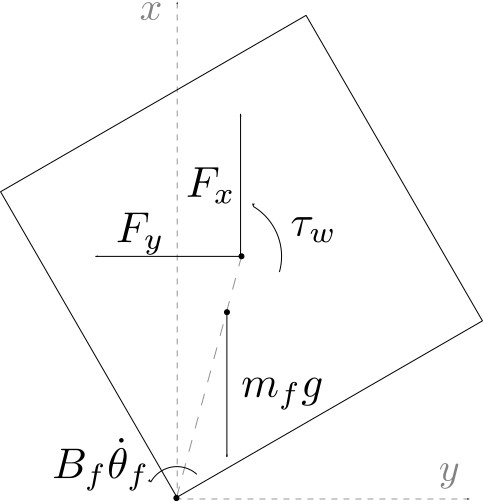
\includegraphics[scale=.5]{figures/freeBodyFrame}
  			\centering
  			\captionsetup{justification=centering}
  			\captionof{figure}{\\Free body diagram of the frame of the cubli}
  			\label{freeBodyFrame}
  		\end{figure}\vspace{-5mm}
  	\end{minipage}
  	\hspace{0.03\linewidth}
  	\begin{minipage}{0.45\linewidth}
  		\begin{figure}[H]
  			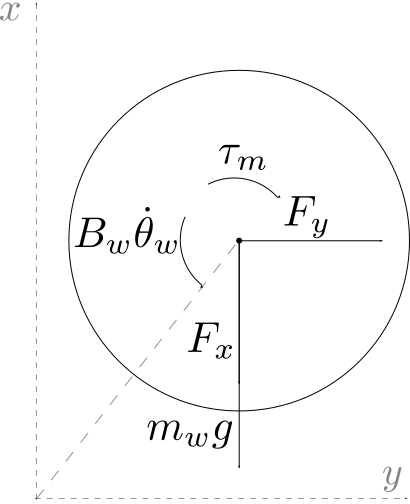
\includegraphics[scale=.53]{figures/freeBodyWheel}
  			\centering
  			\captionsetup{justification=centering}
  			\captionof{figure}{\\Free body diagram of the reaction wheel of the cubli}
  			\label{freeBodyWheel}
  		\end{figure}\vspace{-5mm}
  	\end{minipage}
  \end{minipage}

The equation for the frame is deduced from the \figref{freeBodyFrame}.
\begin{flalign}
  \eq{J_F \vec{\ddot{\theta}_F}} { B_F \vec{\dot{\theta}_F} + \vec{l_F} \times (m_F\cdot \vec{g}) + \vec{l_w} \times \vec{F} - \vec{\tau_w} } \unit{N\cdot m}
  \label{frameModelEq}
\end{flalign}
%
\hspace{6mm} Where:\\
\begin{tabular}{ p{1cm} l l l}
& \si{J_F} 					    	   & is the inertia of the frame                          &\unitWh{kg \cdot m^2} \\
& \si{\vec{\ddot{\theta}_F}} & is the angular acceleration of the frame             &\unitWh{rad \cdot s^{-2}} \\
& \si{\vec{\tau_w}} 	       & is the torque delivered by the reaction wheel        &\unitWh{N \cdot m} \\
& \si{B_F} 	                 & is the friction coefficient of the frame             &\unitWh{N \cdot m \cdot s \cdot rad^{-1}} \\
& \si{\vec{\dot{\theta}_F}}  & is the angular velocity of the frame                 &\unitWh{rad \cdot s^{-1}} \\
& \si{\vec{l_F}}             & is the length to center of mass of the frame         &\unitWh{m} \\
& \si{m_F}                   & is the mass of the frame                             &\unitWh{kg} \\
& \si{\vec{g}}							 & is the gravitational acceleration                    &\unitWh{m\cdot s^{-2}} \\
& \si{\vec{l_w}}             & is the length to center off mass of the wheel        &\unitWh{m} \\
& \si{\vec{F}}				  	   & is the torque delivered to the frame from the wheel  &\unitWh{N}
\end{tabular}

The following equation is then derived from \figref{freeBodyWheel}:
\begin{flalign}
  \eq{ J_w (\ \vec{\ddot{\theta}_F} + \vec{\ddot{\theta}_w}\ ) } { \vec{\tau_m} - B_w \vec{\dot{\theta}_w }} \unit{N\cdot m }
  \label{tauW}
\end{flalign}
\hspace{6mm} Where:\\
\begin{tabular}{ p{1cm} l l l}
& \si{J_w} 					    	   & is the inertia of the wheel                          &\unitWh{kg \cdot m^2} \\
& \si{\vec{\ddot{\theta}_w}} & is the angular acceleration of the wheel             &\unitWh{rad \cdot s^{-2}} \\
& \si{\vec{\tau_m}} 	       & is the torque delivered by the motor                 &\unitWh{N \cdot m} \\
& \si{B_w}                   & is the friction coefficient of the wheel          &\unitWh{N \cdot m \cdot s \cdot rad^{-1}} \\
& \si{\vec{\dot{\theta}_w}}  & is the angular velocity of the wheel                 &\unitWh{rad \cdot s^{-1}}
\end{tabular}

In \eqref{frameModelEq} the term \si{\vec{l_w} \times \vec{F}} describes the the torque delivered from the wheel to the frame, as it acts around the pivot corner of the frame. The vector \si{\vec{F}} is composed of the two linear forces \si{F_x} and \si{F_y}, as seen on \figref{freeBodyFrame} and \figref{freeBodyWheel}. To further investigate these two forces, expressions for both the x- and y-coordinate describing the position of the center of mass of the wheel are found.
%
\begin{flalign}
  \eq{x} { lw \cdot cos( \theta_F ) } \unit{ m }\\
  \eq{y} { lw \cdot sin( \theta_F ) } \unit{ m }
  \label{xyCoordinate}
\end{flalign}
%
According to Newton's 2nd law of motion, \si{\sum F = m \cdot a}. Then to find \si{F_x} and \si{F_y}, the acceleration of the point at center of mass of the wheel must be known for both the x- and the y-direction. To achieve this the derivatives of the expressions for x and y in \eqref{xyCoordinate} are derived.
%
\begin{flalign}
  \eq{\dot{x}} { -lw \cdot sin( \theta_F )\ \dot{\theta}_F } \unit{ m\cdot s^{-1} }\\
  \eq{\ddot{x}} { -lw \cdot cos( \theta_F )\ {\dot{\theta}_F}^{\ \ 2} - lw \cdot sin( \theta_F ) \ddot{\theta}_F } \unit{ m\cdot s^{-2} }
  \label{xCoordinateDerivatives}
\end{flalign}
%
\begin{flalign}
  \eq{\dot{y}} { lw \cdot cos( \theta_F )\ \dot{\theta}_F } \unit{ m\cdot s^{-1} }\\
  \eq{\ddot{y}} { -lw \cdot sin( \theta_F )\ {\dot{\theta}_F}^{\ \ 2} + lw \cdot cos( \theta_F )\ \ddot{\theta}_F } \unit{ m\cdot s^{-2} }
  \label{yCoordinateDerivatives}
\end{flalign}
%
\Eqref{xCoordinateDerivatives} and \eqref{yCoordinateDerivatives} can now be used with Newton's 2nd law of motion, while also taking gravity into account in sum of forces, to derive \si{F_x} and \si{F_y}.
%
\begin{flalign}
  \eq{ -F_x -m_w \cdot g }{ m_w \cdot \ddot{x} } &\nonumber\\
  \eq{ F_x }{ - m_w \cdot \ddot{x} - m_w \cdot g} &\nonumber\\
  \eq{ F_x }{ m_w \cdot (\  lw \cdot cos( \theta_F )\ {\dot{\theta}_F}^{\ \ 2} + lw \cdot sin( \theta_F )\ \ddot{\theta}_F \ ) - m_w \cdot g} \unit{N}
  \label{Fx}
\end{flalign}
%
\begin{flalign}
  \eq{ F_y }{ m_w \cdot \ddot{y} } & \nonumber\\
  \eq{ F_y }{ m_w \cdot (\ -lw \cdot sin( \theta_F )\ {\dot{\theta}_F}^{\ \ 2} + lw \cdot cos( \theta_F )\ \ddot{\theta}_F\ ) } \unit{N}
  \label{Fy}
\end{flalign}

The original objective was to evaluate the term \si{\vec{l_w} \times \vec{F}} in \eqref{frameModelEq}. Since the expressions for the two forces, \si{F_x} and \si{F_y}, composing the vector \si{\vec{F}}, are found in \eqrefTwo{Fx}{Fy}, the vector product from \eqref{frameModelEq} is evaluated.

\begin{flalign}
  \si{\vec{l_w} \times \vec{F}} &=
    \begin{vmatrix}
      \ \si{\vec{\hat{i}}}                & \si{\vec{\hat{j}}}               & \si{\vec{\hat{k}}} \ \ \ \\ 
      \ \si{ l_w \cdot cos( \theta_F ) }  & \si{ l_w \cdot sin( \theta_F ) } & 0                  \ \ \ \\ 
      \ \si{ F_x }                        & \si{ -F_y }                      & 0                  \ \ \  
    \end{vmatrix} \unit{N\cdot m}\\ \nonumber \\
  \si{ \vec{l_w} \times \vec{F} } &= 
    \begin{bmatrix}
      \ \si{ ( l_w \cdot sin( \theta_F) \cdot 0 - 0 \cdot -F_y ) } \ \ \ \\
      \ \si{ ( l_w \cdot cos( \theta_F )\cdot 0 + 0 \cdot F_x  ) } \ \ \ \\
      \ \si{ ( l_w \cdot cos( \theta_F )\cdot -F_y - lw \cdot sin( \theta_F )\cdot F_x ) }
    \end{bmatrix} \unit{N\cdot m} \\ \nonumber\\
  \si{ \vec{l_w} \times \vec{F} } &= \si{( lw \cdot cos( \theta_F )\cdot (m_w \cdot (\ lw \cdot sin( \theta_F )\ {\dot{\theta}_F}^{\ \ 2} - lw \cdot cos( \theta_F )\ \ddot{\theta}_F\ ))} \nonumber \\
  &\ \ \ \si{- lw \cdot sin( \theta_F )\cdot (m_w \cdot (\  lw \ cos( \theta_F )\ {\dot{\theta}_F}^{\ \ 2} + lw \cdot sin( \theta_F )\ \ddot{\theta}_F \ )} \nonumber \\
  &\ \ \ \si{- m_w \cdot g) ) \cdot \hat{k}} \unit{N \cdot m}\\ \nonumber\\
  \eq{ \vec{l_w} \times \vec{F} }{ {l_w}^2 \cdot m_w \ddot{\theta}_F \ (cos^2(\theta_F) + sin^2(\theta_F)) + l_w\cdot sin(\theta_F)\ m_w \cdot g } \unit{N \cdot m}\\ \nonumber\\
  \eq{ \vec{l_w} \times \vec{F} }{ {l_w}^2 \cdot m_w \ddot{\theta}_F + l_w\ sin(\theta_F)\ m_w \cdot g } \unit{N \cdot m}
  \label{vectorDecomposition3}
\end{flalign}

Since all torques are represented in z-coordinate, \eqref{vectorDecomposition3} is inserted in \eqref{frameModelEq}, without vector-notation. Note that \si{\vec{l_F} \times (m_F\cdot \vec{g}) = m_F \cdot l_F \cdot g \cdot sin(\theta_F) }.
%
\begin{flalign}
	J_F \cdot \ddot{\theta}_F &= - B_F \cdot \dot{\theta}_F + m_F \cdot l_F \cdot g \cdot sin(\theta_F) \nonumber\\ 
	&- m_w \cdot {l_w}^{2} \cdot \ddot{\theta}_F + m_w \cdot l_w  \cdot g \cdot sin(\theta_F) - \tau_w \unit{N \cdot m} 
\label{FrameEq2}
\end{flalign}
%
\begin{flalign}
	\eq{(J_F+m_w \cdot {l_w}^{2}) \cdot \ddot{\theta}_F} {- B_F \cdot \dot{\theta}_F + (m_F \cdot l_F + m_w \cdot l_w) \cdot g \cdot sin(\theta_F) - \tau_w}  \unit{N \cdot m} 
\label{FrameEq3}
\end{flalign}

Note that \si{\tau_w=\tau_m-B_w \cdot \dot{\theta}_w}.
\begin{flalign}
	(J_F+m_w \cdot {l_w}^{2}) \cdot \ddot{\theta}_F &= - B_F \cdot \dot{\theta}_F + (m_F \cdot l_F + m_w \cdot l_w) \cdot g \cdot sin(\theta_F) \nonumber\\ 
	&- \tau_M + B_w \cdot \dot{\theta}_w  \unit{N \cdot m} 
\label{FrameEq4}
\end{flalign}

Isolating \si{\ddot{\theta}_F} from \eqref{FrameEq4} gives the final expression for the rotational acceleration of the frame.
\begin{flalign}
	\eq{\ddot{\theta}_F} {\frac{- B_F \cdot \dot{\theta}_F + (m_F \cdot l_F + m_w \cdot l_w) \cdot g \cdot sin(\theta_F) - \tau_M + B_w \cdot \dot{\theta}_w}{J_F + m_w \cdot {l_w}^{2}}}  \unit{rad \cdot s^{-1}} 
\label{FrameEqFinal}
\end{flalign}

Once the acceleration of the frame is described by \eqref{FrameEqFinal} it is possible to derive an expression for the angular acceleration of the wheel with respect to its axis from \eqref{tauW}.
\begin{flalign}
	\eq{\ddot{\theta}_w} {\frac{\tau_m - B_w \cdot \dot{\theta}_w}{J_w} - \ddot{\theta}_F} \unit{rad \cdot s^{-1}} 
\label{WheelRotEq2}
\end{flalign}

Substituting \si{\ddot{\theta}_F} by the expression for the angular acceleration of the frame (\eqref{FrameEqFinal}) into \eqref{WheelRotEq2} gives the final description for \si{\ddot{\theta}_w}, as shown in \eqref{WheelRotEqFinal}.
\begin{flalign}
	\ddot{\theta}_w &= \frac{\tau_m - B_w \cdot \dot{\theta}_w}{J_w}\nonumber\\ 
	&- \frac{(m_F \cdot l_F + m_w \cdot l_w) \cdot g \cdot sin(\theta_F) - \tau_M + B_w \cdot \dot{\theta}_w - B_F \cdot \dot{\theta}_F}{J_F+m_w \cdot {l_w}^{2}} \unit{rad \cdot s^{-1}} 
\label{WheelRotEq3}
\end{flalign}
%
\begin{flalign}
	\ddot{\theta}_w &= \frac{(J_w+J_F+{l_w}^{2} \cdot m_w) \cdot (\tau_m - B_w \cdot \dot{\theta}_w)}{J_w \cdot (J_F+m_w \cdot {l_w}^{2})}\nonumber\\ 
	&- \frac{(m_F \cdot l_F + m_w \cdot l_w) \cdot g \cdot sin(\theta_F) - B_F \cdot \dot{\theta}_F}{J_F+m_w \cdot {l_w}^{2}} \unit{rad \cdot s^{-1}} 
\label{WheelRotEqFinal}
\end{flalign}             %-------- Model
\section{Linearization of the Model}
Now that a model of the Cubli frame is put forth in \eqref{FrameEqFinal}, it is apparent that the system is nonlinear due to the term including \si{sin(\theta_F)}. In order to proceed with a simulation and controller design, it is convenient to first linearize the model. This is done by use of a Taylor series approximation.

Based on \eqref{FrameEq3} the system is described in an operating point, around which it varies with \si{\Delta \theta_F}.
%
\begin{flalign}
	\si{(J_F+m_w \cdot {l_w}^{2}) (\ddot{\theta}_F + \Delta \ddot{\theta}_F )} &= \si{- B_F \cdot (\dot{\theta}_F + \Delta \dot{\theta}_F) }   \nonumber\\
	&\ \ \ \ \si{+ (m_F \cdot l_F + m_w \cdot l_w) \cdot g \cdot sin(\theta_F + \Delta \theta_F)} \nonumber\\
	&\ \ \ \ \si{- \tau_M + B_w \cdot \dot{\theta}_w}  \unit{N \cdot m}\\
	\eq{(J_F+m_w \cdot {l_w}^{2}) (\ddot{\theta}_F + \Delta \ddot{\theta}_F )}{ f( (\dot{\theta}_F + \Delta \dot{\theta}_F), \ (\theta_F + \Delta \theta_F), \ (\tau_m + \Delta \tau_m),\  (\dot{\theta}_w + \Delta \dot{\theta}_w) ) } \unit{N \cdot m}
\label{FrameEq4OperatingPoint}
\end{flalign}
%
The operating point is chosen to be \si{\theta_F = 0}, which corresponds to the frame being in upright position, see \figref{cubliMechanical}. Taking this into account and applying the Taylor series approximation yields the following.
%
\begin{flalign}
	\si{(J_F+m_w \cdot {l_w}^{2}) \Delta \ddot{\theta}_F } &= \cancelto{0}{\si{f( \dot{\theta}_F, \ \theta_F, \ \tau_m,\ \ddot{\theta}_w )}}   \nonumber\\
	&\ \ \ \ \si{+ \frac{\partial}{\partial \dot{\theta}_F} f\cdot \Delta \dot{\theta}_F + \frac{\partial}{\partial \theta_F} f\cdot \Delta \theta_F + \frac{\partial}{\partial \tau_m} f\cdot \Delta \tau_m + \frac{\partial}{\partial \dot{\theta}_w} f\cdot \Delta \dot{\theta}_w } \unit{N \cdot m}
\label{FrameEq4OperatingPointZero}
\end{flalign}

All the higher order derivatives are discarded due to their negligible impact on the system when it is near the operating point.
%
\begin{flalign}
	\si{(J_F+m_w \cdot {l_w}^{2}) \Delta \ddot{\theta}_F } &= \si{-B_F \Delta \dot{\theta}_F +  ( m_F \cdot l_F + m_w \cdot l_w ) g \cdot} \cancelto{1}{\rule{0cm}{.4cm} \si{  cos(\theta_F)}} \si{\Delta \theta_F} \where{\theta_F = 0} \nonumber\\
	&\ \ \ \ \si{- \Delta \tau_m + B_w \Delta \dot{\theta}_w } \unit{N \cdot m}\\
	\eq{(J_F+m_w \cdot {l_w}^{2}) \Delta \ddot{\theta}_F }{-B_F \Delta \dot{\theta}_F +  ( m_F \cdot l_F + m_w \cdot l_w ) g \cdot \Delta \theta_F - \Delta \tau_m + B_w \Delta \dot{\theta}_w } \unit{N \cdot m}
\label{FrameEq4TaylerApprox}
\end{flalign}
%
\Eqref{FrameEq4TaylerApprox} shows the final linearized model.

\begin{figure}[H] 
	\centering 
	\includegraphics[scale=1.5]{figures/linearizationPoint}
	\caption{Sketch of linearization for the Cubli frame angels.}
	\label{LinearizationSketch}
\end{figure} 

Due to the linearization of the model there will be an point where the controller will no longer be able to catch the frame, because it cannot predict the forces on the frame anymore. In the sketch (see \figref{LinearizationSketch}) the area where the controller will work is indicated by the green area.    %-------- Linearization
\section{Verification of the Model}

To verify the model in simulation \eqref{FrameEq4TaylerApprox} is transformed into the Laplace domain, after which a transfer function of the system is derived. The proceeding equations are valid only around the operating point, and so for better overview, in the following \si{\Delta \theta_F = \theta_F}.
%
\begin{flalign}
	\eq{(J_F+m_w \cdot {l_w}^{2}) \cdot \theta_F \cdot s^2}{-B_F \theta_F\cdot s +  ( m_F \cdot l_F + m_w \cdot l_w ) g \cdot \theta_F - \tau_m + B_w \theta_w\cdot s } \unit{N \cdot m}
\label{LaplaceOfLinearizedModel}
\end{flalign}
%
The angle of the reaction wheel, \si{\theta_w}, still features in \eqref{LaplaceOfLinearizedModel}. It is desireable to have only one input, \si{\tau_m}, and one output, \si{\theta_F}. To achieve this, \eqref{WheelRotEq2} is transformed into the Laplace domain and solved for \si{\theta_w}.
%
\begin{flalign}
	\eq{\theta_w\cdot s^2} {\frac{\tau_m - B_w \theta_w\cdot s}{J_w} - \theta_F\cdot s^2}   &\\
	\eq{\theta_w} {\frac{ -J_w \theta_F \cdot s^2 + \tau_m }{ J_w \cdot s^2 + B_w \cdot s }}&
\label{WheelRotEq2Laplace}
\end{flalign}
%
\Eqref{WheelRotEq2Laplace} is now substituted for \si{\theta_w} in \eqref{LaplaceOfLinearizedModel}, and the transfer function is of the system is derived.
%
\begin{flalign}
	\si{(J_F+m_w \cdot {l_w}^{2}) \cdot \theta_F \cdot s^2} &= \si{-B_F \theta_F\cdot s +  ( m_F \cdot l_F + m_w \cdot l_w ) g \cdot \theta_F - \tau_m} &\nonumber\\
	&\ \ \ \ \si{+ B_w ( \frac{ -J_w \theta_F \cdot s^2 + \tau_m }{ J_w \cdot s^2 + B_w \cdot s } )\cdot s }&
\label{CubliTransferFunction}
\end{flalign}    %-------- Verification

%---------- Chapter 5 ---------------------------------------- Control
%\chapter{System Modelling}
With the given setup \fxnote{Fix this once we have agreed on a name for the cubli thingy} being described, it is necessary to study its natural behavior in more details by deriving a model of this system. This chapter shows the process used to put up this model and an analysis of its pertinence. With this model, it shall be possible to determine realistic requirements for the controllers to implement in this project, see \chapref{chap:requirements} \fxnote{check that this actually refers to requirements}.

As a start to this modelling, a mechanical drawing of the Cubli showing angles and coordinate system conventions is seen in \figref{cubliMechanical}. A two-dimensional global coordinate system is chosen with its origin on the pivot point of the frame. Moreover, angles of the total body and the wheel count grow clockwise.

\begin{figure}[H]
 \centering
 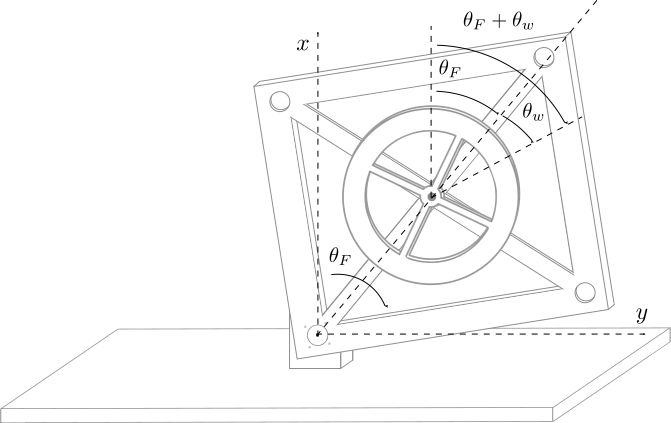
\includegraphics[scale=0.6]{figures/mechanicalSystem}
 \caption{Mechanical drawing of the Cubli, including angle coordinate system conventions}
 \label{cubliMechanical}
\end{figure}

%As shown in \figref{cubliMechanical}, 
In the next section, a complete model of the given setup is derived from Newton's Second Law of motion and rotation.

%%% Part 3 %%%
\part{Test \& Conclusion}
%\input{chapters/aAcceptanceTest/AcceptanceTest}
%\chapter{Conclusion}

The aim of this project was to work with an unstable nonlinear system and be able to construct an appropriate model and design a controller capable of balancing it around equilibrium position.

First, a pre-analysis of the system has been made, starting from a description of all the components present in the given setup. It also included the derivation of the equations that describe the dynamics and the description of the system in s-domain. Then the parameters of the setup have been found, both with measurements and with an estimation using optimization, to be able to analyze the behavior of the system and compare it with the real model.

Afterwards, a controller has been designed to balance the Cubli in upright position using root locus. It has been shown necessary to control both the angular position of the frame and the velocity of the wheel so it was decided to use a state space approach.

It was also a requirement to be able to change the angle of the baseplate, which means that the calculation of the angle had to be independent of the inclination. A very convenient option was to use built-in sensors for this purpose, so the final chosen solution was to use an IMU present on the setup and calculate the angle through a complementary filter.

Finally, some acceptance tests have been performed to ensure that the final controlled system was able to accomplish the requirements and, similarly, a further analysis has been carried out to check other capabilities of the Cubli.

In conclusion, a control system that can balance the Cubli in upright position independently of the angle of the baseplate, within a reasonable range, has been designed, implemented and tested successfully within the requirements.

%\chapter{Discussion}

{\Large notes} \fxnote{delete this part its just to brainstorm what to write in this section}\\
- Placement of IMU\\
- Choice of Statspace variables for controller - minimize overshoot vs faster braking for wheel\\
- cut-off frequency of the complementary filter?\\
- 
- 


As already mentioned briefly in the complementary section the measurement from the accelerometer in the IMU could be improved by moving the sensor to a position where it would be influenced less by the acceleration of the frame but still be able to measure the angle of the frame. 



%%% Setup for Appendix and Bibliography %%%
\bookmarksetup{startatroot}
\addtocontents{toc}{\bigskip}
\newpage
\fancyhead[RO]{\color{aaublue}\small Appendix \nouppercase\rightmark} %even page - chapter title
\fancyhead[LE]{\color{aaublue}\small Appendix \nouppercase\rightmark} %uneven page - section title
\fancyhead[RE,LO]{}
\titleformat{\section}[hang]{\Large\bfseries}{\thesection\hsp\textcolor{aaublue}{|}\hsp}{0pt}{\Large\bfseries}
\renewcommand{\thechapter}{\Alph{chapter}}
\setcounter{chapter}{0}

%%% Appendix %%%
\part*{Appendix}
\addcontentsline{toc}{chapter}{Appendix}

%---------- Appendix A ---------------------------------------- Test Title
\chapter{Fall Response}\label{comparisonLinModelReal} 
\textbf{Name: Group 630}\\
\textbf{Date: 07/03 - 2016}

\subsubsection{Purpose}
Find the fall response of the frame from the vertical position, \si{\theta_F=0}\fxnote{might change depending on what is decided as the "real" 0 because of potmeter offset}, and from a \si{10^\circ}\fxnote{Might chance depending on data } tilted position. During this the wheel will be in a fixed position.

Data from this is used to compare the response of the real setup with the simulation given by the theoretical linearized model.

\subsubsection{Setup}
The wheel is being held in a fixed position with a strip tied to it and the frame. The probe chosen is a 1:1 and is connected to the potentiometer with probe to yellow cable and ground clamp to brown cable. The power supply has to be connected, and turned on, to the Cubli in order to get readouts from the potentiometer. A sponge is placed on the rubber pad in order to dampen the impact of the frame.
\begin{figure}[H]                                   
	\centering                                        
	\includegraphics[scale=0.08]{figures/stepResponseSetup}
	\caption{Picture of the setup for the step-response test}
	\label{stepResponseTestPicture} 
\end{figure}              

\subsubsection{List of Equipment}
\begin{table}[H]
	\begin{tabular}{|l|l|p{4cm}|}
		\hline%------------------------------------------------------------------------------------
		\textbf{Instrument}                        &  \textbf{AAU-no.}  &  \textbf{Type}       \\
		\hline%------------------------------------------------------------------------------------
		Oscilloscope                              &  61604             &  Agilent 54621A		  \\
		\hline%------------------------------------------------------------------------------------
		Dedicated Power Supply of Cubli \small{(24 V - 3 A)} &               &  XP Power, AEB70US24 \\
		\hline%------------------------------------------------------------------------------------
		Probe 1:1                &  TBD            &          TBD\fxnote{find the probe used}    \\
		\hline%------------------------------------------------------------------------------------
		Sponge               &              &              \\
		\hline%------------------------------------------------------------------------------------
	\end{tabular}
\end{table}
>>>>>>> b5c3798a86deb9e8a1f72534e3bf37d900175072

\subsubsection{Procedure}
\begin{enumerate}
	%\item Turn on the power supply
	\item Keep the Cubli near the starting position (\si{0^\circ} or \si{10^\circ})
	\item Let the Cubli fall over
	\item Use the oscilloscope to measure the voltage changes in the potentiometer and save them
	\item Take the measurements and plot them in Matlab
	%\item Plot the result of the simulations in the same figure and compare them

\end{enumerate}

%\subsubsection{Results}
%\begin{figure}[H] 
%	\centering 
%	\includegraphics[scale=0.9]{figures/comparisonRealModel}
%	\caption{Comparison between the real behavior and the simulation of the linearized model}
%	\label{rawDataFallResponse}
%\end{figure} 

\begin{minipage}{\linewidth}
	\begin{minipage}{0.45\linewidth}
		\begin{figure}[H]
			\includegraphics[scale=.53]{figures/comparisonRealModel}
			\centering
			\vspace{-.4cm}
			\captionsetup{justification=centering}
			\captionof{figure}{FIGURE 1 description}
			\label{HbridgeClokwise4Q}
		\end{figure}\vspace{-5mm}
	\end{minipage}
	\hspace{0.03\linewidth}
	\begin{minipage}{0.45\linewidth}
		\begin{figure}[H]
			\includegraphics[scale=.53]{figures/comparisonRealModel}
			\centering
			\vspace{-.4cm}
			\captionsetup{justification=centering}
			\captionof{figure}{figure 2 description}
			\label{HbridgeCounterClokwise4Q}
		\end{figure}\vspace{-5mm}
	\end{minipage}
\end{minipage} \fxnote{Look at the layout of picture of data placement}

The data is available as a .csv file on the CD\fxnote{Make sure this is put into the CD folder for copying}

%The result of the experiment (\figref{comparisonRealModel}) shows that the response of the real system has several differences with the one from the simulation.
%
%The fist one is the presence of oscillations in the real response curve. This behavior is due to a small bounce that the frame does when it reaches the base.
%
%Another one is the final position of the frame, but it is due to the existence of a piece of foam at this position in the real case (to avoid the Cubli to hit the base).
%
%The other main difference is the shape of the curve, since the simulation is slower than the real case.

\subsubsection{Note}
Because of the sponge used as a cushion, to dampen the impact of the Cubli, there can be observed some bouncing in the data when the frame reaches the outer position.

\subsubsection{Conclusions}



%---------- Appendix B ---------------------------------------- Test Title
%\chapter{Impulse Response}\label{comparisonModelReal} 
\textbf{Name: Group 630}\\
\textbf{Date: 11/03 - 2016}

\subsubsection{Purpose}
To observe the impulse response of the Cubli hanging upside down.

Data is used to compare the response of measured response and the simulation given by the theoretical nonlinear model.

\subsubsection{Setup}
\begin{figure}[H] 
	\centering 
	\includegraphics[scale=0.1]{figures/impulseResponseSetup}
	\caption{The Cubli setup hanging upside down beneath a table during the impulse response test}
	\label{impulseResponseTestPicture}
\end{figure} 

\subsubsection{Procedure}
\begin{enumerate}
	\item Turn on the power supply
	\item Place the setup upside-down and place the frame touching the base, \si{135^0} with respect to the vertical position
	\item Use the oscilloscope to measure the changes in the potentiometer 
	\item Let the Cubli fall
	\item Collect all the data and plot it in Matlab
	\item Compare with the simulation 
	
\end{enumerate}

\subsubsection{Results}
\begin{figure}[H] 
	\centering 
	\includegraphics[scale=0.9]{figures/comparisonRealModel}
	\caption{Comparison between the real behavior and the simulation of the linearized model}
	\label{comparisonRealModel}
\end{figure} 

\subsubsection{Conclusions}

%----------Appendix C ---------------------------------------- Test Title
%\input{appendix/cTest.tex}

%---------- Appendix D ---------------------------------------- Test Title
%\input{appendix/dTest.tex}

%%% Bibliography %%%
\printbibliography

%%% To Do List %%%

\end{document}
